
% Asset ID: A21RadiansTikZ-006
% Purpose: Show a radian interval for solving trig equations such as sin(3 theta)=sqrt(3)/2.
\documentclass[tikz,border=8pt]{standalone}
\usetikzlibrary{arrows.meta}
\begin{document}
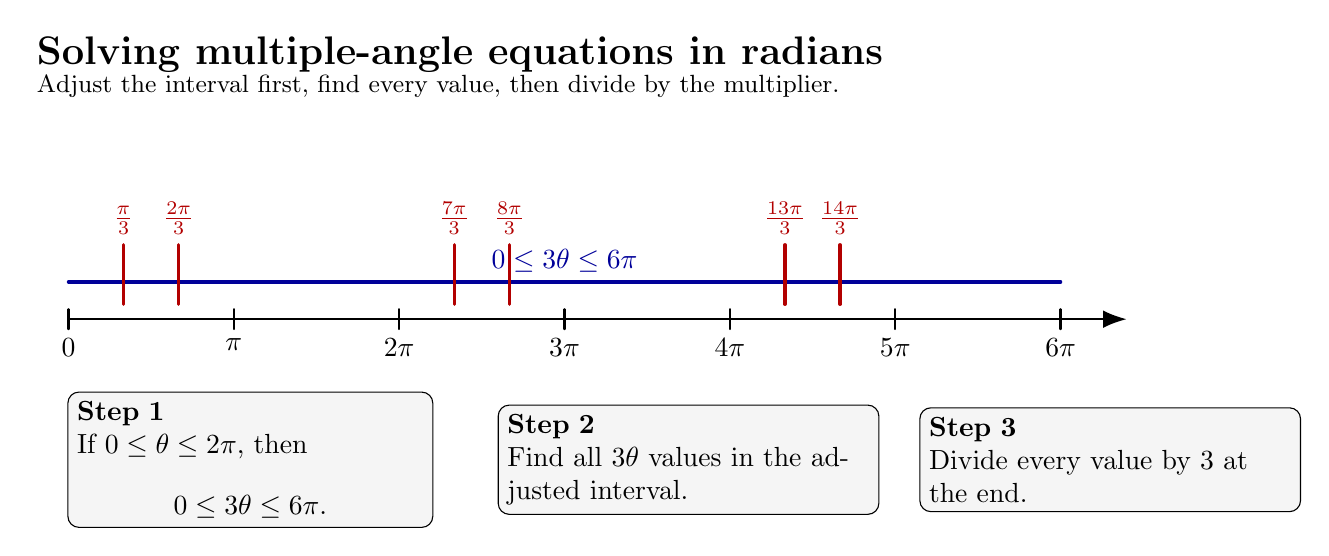
\begin{tikzpicture}[scale=1.05,line cap=round,line join=round]
\node[anchor=west,font=\bfseries\Large] at (-0.5,3.2) {Solving multiple-angle equations in radians};
\node[anchor=west,font=\small] at (-0.5,2.82) {Adjust the interval first, find every value, then divide by the multiplier.};
\draw[-{Latex[length=3mm]},thick] (0,0)--(12.8,0);
\foreach \x/\lab in {0/\(0\),2/\(\pi\),4/\(2\pi\),6/\(3\pi\),8/\(4\pi\),10/\(5\pi\),12/\(6\pi\)}{\draw[thick] (\x,0.12)--(\x,-0.12);\node[below] at (\x,-0.12) {\lab};}
\draw[blue!60!black,very thick] (0,0.45)--(12,0.45);\node[above,blue!60!black] at (6,0.45) {\(0\leq 3\theta\leq 6\pi\)};
\foreach \x/\lab in {0.666/\(\frac{\pi}{3}\),1.333/\(\frac{2\pi}{3}\),4.666/\(\frac{7\pi}{3}\),5.333/\(\frac{8\pi}{3}\),8.666/\(\frac{13\pi}{3}\),9.333/\(\frac{14\pi}{3}\)}{\draw[red!70!black,very thick] (\x,0.18)--(\x,0.9);\node[above,red!70!black] at (\x,0.9) {\lab};}
\node[draw,rounded corners,fill=gray!8,align=left,text width=4.4cm] at (2.2,-1.7) {\textbf{Step 1}\\If \(0\leq\theta\leq2\pi\), then\[0\leq3\theta\leq6\pi.\]};
\node[draw,rounded corners,fill=gray!8,align=left,text width=4.6cm] at (7.5,-1.7) {\textbf{Step 2}\\Find all \(3\theta\) values in the adjusted interval.};
\node[draw,rounded corners,fill=gray!8,align=left,text width=4.6cm] at (12.6,-1.7) {\textbf{Step 3}\\Divide every value by \(3\) at the end.};
\end{tikzpicture}
\end{document}
